\uuid{VbQK}
\exo7id{7167}
\titre{exo7 7167}
\auteur{megy}
\organisation{exo7}
\datecreate{2017-07-08}
\isIndication{false}
\isCorrection{true}
\chapitre{Géométrie affine euclidienne}
\sousChapitre{Géométrie affine euclidienne du plan}
\module{Géométrie}
\niveau{L2}
\difficulte{}

\contenu{
\texte{
% rotations
Soient $AOB$ et $COD$ deux triangles directs, isocèles rectangles en $O$. Soient $I$, $J$, $K$ et $L$ les milieux des segments $[AB]$, $[BC]$, $[CD]$ et $[DA]$.

\begin{center}
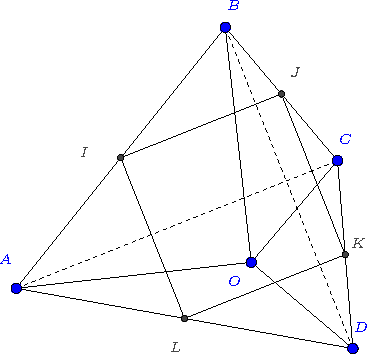
\includegraphics{../images/pdf/VbQK-1.pdf}
\end{center}
}
\begin{enumerate}
    \item \question{Montrer que $(AC)\bot (BD)$ et que $AC=BD$.}
\reponse{Soit $\rho$ la rotation de centre $O$ et d'angle $\pi/2$. D'après l'énoncé, on a $\rho(B)=A$ et $\rho(D)=C$. Donc $[AC]$ est l'image de $[AD]$ par $\rho$, d'où on déduit que $(AC)\bot (BD)$ et que $AC=BD$.}
    \item \question{Montrer que $IJKL$ est un carré.}
\reponse{Le quadrilatère $IJKL$ est toujours un parallélogramme, même sans hypothèses sur $ABCD$ (c'est le théorème de Varignon). En effet, par le théorème de Thalès (ou simplement le théorème des milieux) : 
\[ \overrightarrow{IL} = \frac12 \overrightarrow{BD} = \overrightarrow{JK}.\]
Ceci signifie que les côtés $[IL]$ et $[JK]$ ont même longueur et sont parallèles, donc $IJKL$ est un parallélogramme.

Pour voir que c'est un carré, remarquons qu'on montre de même que  
\[ \overrightarrow{IJ} = \frac12 \overrightarrow{AC} = \overrightarrow{LK},\]
et d'après la première question, $(AC)\bot (BD)$ et que $AC=BD$, donc $IJKL$ est un parallélogramme ayant un angle droit et des cotés consécutifs de même longueur. C'est donc un carré.}
\end{enumerate}
}
